\documentclass{article}

\usepackage[dutch]{babel}
\usepackage[margin=3cm]{geometry}
\usepackage{graphicx}
\usepackage{float}
\usepackage{caption}
\usepackage{hyperref}
\usepackage{amsmath}
\usepackage{wrapfig}
\usepackage[parfill]{parskip}

% fonts
\usepackage[T1]{fontenc}
\usepackage{helvet}
\renewcommand{\familydefault}{\sfdefault}

\graphicspath{{img/}}
 
\newcommand{\bold}[1]{\textbf{#1}}

\usepackage{minted}
\usepackage{upquote}
\usepackage{color}

\begin{document}

\begin{titlepage}
    \author{Tuur Vanhoutte}
    \title{Big Data - Labo}
\end{titlepage}

\pagenumbering{gobble}
\maketitle
\newpage
\tableofcontents
\newpage

\pagenumbering{arabic}

\section{Intro}

Topics:

\begin{itemize}
    \item Linux basics + containers
    \item Elastic search (text search, document store)
    \item Linux Batch Processing \& Dask
    \item InfluxDB (timeseries)
    \item Cloud services (Kafka, Kinesis, Lambda, ML services, \dots)
\end{itemize}

\section{NAT-ing}

\subsection{NAT}

= Network Address Translation

\begin{figure}[H]
    \centering
    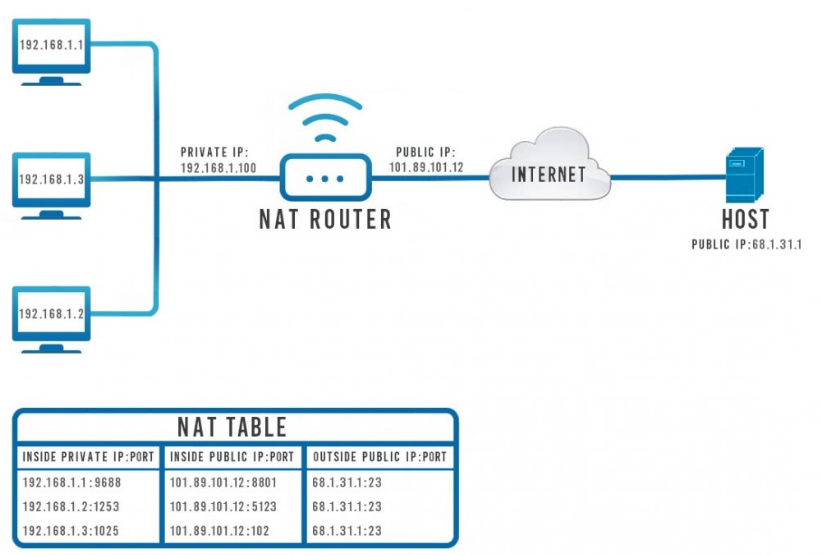
\includegraphics[width=0.5\textwidth]{nat.png}
    \caption{NAT diagram}
\end{figure}

\subsubsection{The problem}

\begin{itemize}
    \item We only have one (public/private) IP-address
    \begin{itemize}
        \item Howest: 172.23.82.60
    \end{itemize}
    \item Connecting to a server over a network:
    \begin{itemize}
        \item Using a protocol (HTTP) which uses TCP
        \item Our server has an IP address: 172.23.82.60
        \item Our server is listening at port 5000
        \item $\Rightarrow$ \url{http://172.23.82.60:5000}
    \end{itemize}
    \item Problem: We want to have multiple IP addresses
    \begin{itemize}
        \item Student 1 wants to reach http://192.168.20.21:5000
        \item Student 2 wants to reach http://192.168.20.22:5000
        \item Student x  wants to reach http://192.168.20.xx:5000
    \end{itemize}
\end{itemize}

\subsubsection{The solution}

Translation is needed!

\begin{itemize}
    \item 172.23.82.60:5000 should point to 192.168.20.21:5000
    \item 172.23.82.60:5001 should point to 192.168.20.22:5000
    \item 172.23.82.60:5xxx should point to 192.168.20.xx:5000
\end{itemize}

We can use any port, on both sides:

\begin{itemize}
    \item 172.23.82.60:8000 can point to 192.168.20.21:5000
    \item 172.23.82.60:8000 can point to 192.168.20.21:3000
\end{itemize}

\subsection{SSH Tunnel}

= SSH Port Forwarding

\begin{figure}[H]
    \centering
    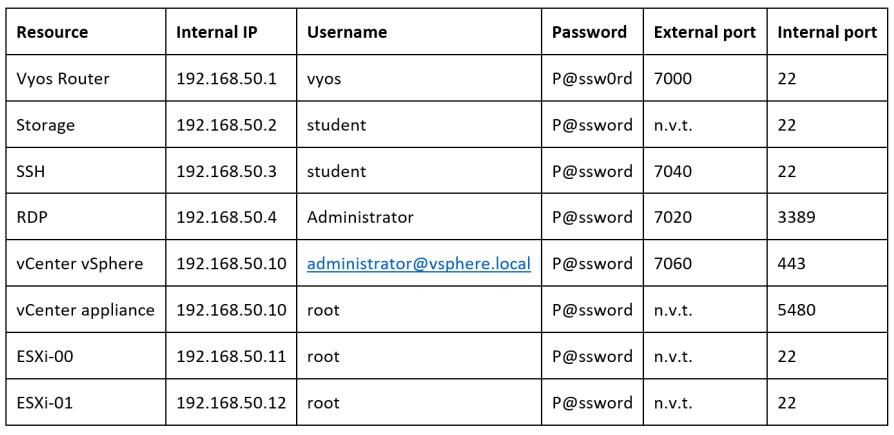
\includegraphics[width=0.5\textwidth]{ssh-tunnel.png}
    \caption{Example}
\end{figure}

\begin{figure}[H]
    \centering
    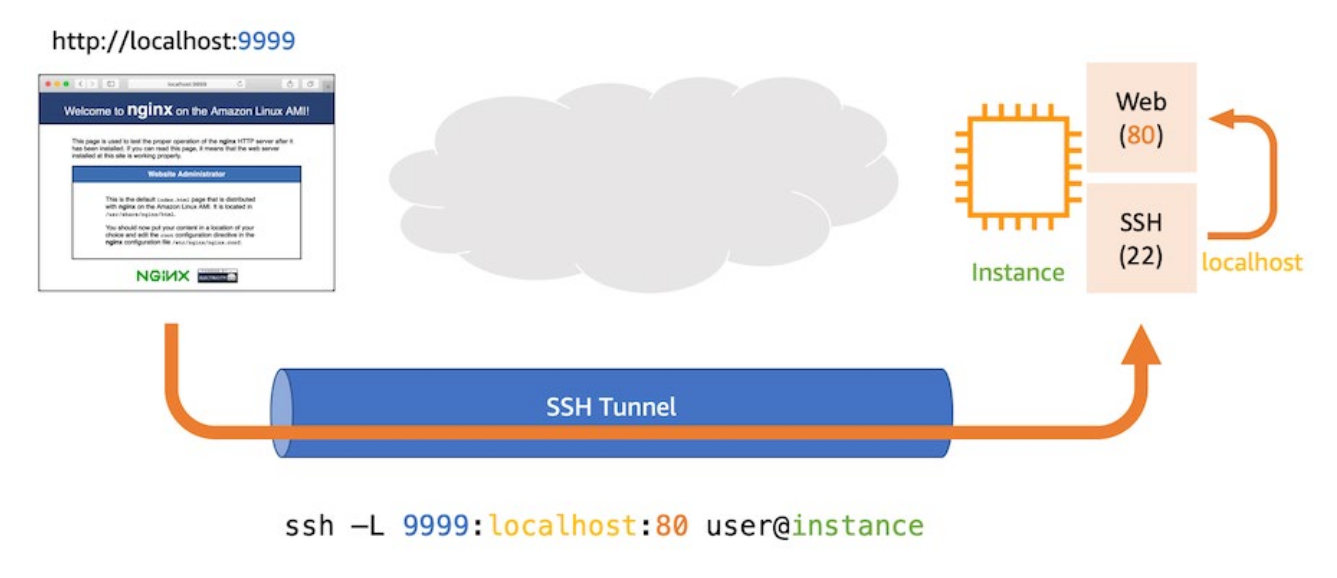
\includegraphics[width=0.7\textwidth]{ssh-tunnel2.png}
    \caption{Voorbeeld: een tunnel wordt opengemaakt en er wordt ingelogd in user@instance}
\end{figure}


\section{Container technology}

\subsection{Docker}

\begin{itemize}
    \item Docker = ecosystem for creating and running containers
    \item Docker wants to make it possible to install and run software on any system
    \item Other reasons: Microservices/DevOps/Resource usage
    \item Docker != Container
    \begin{itemize}
        \item Docker CLI
        \item Docker Engine
        \item Docker Image
        \item Docker Container
        \item Docker Hub
        \item Docker Compose
        \item Docker Swarm
        \item \dots
    \end{itemize}
\end{itemize}

\subsection{Microservices}

\begin{itemize}
    \item = A software development technique
    \item Structure an application as a collection of loosely coupled services
    \item Lightweight
    \item Microservices-based architectures enable continuous delivery and deployment
    \item \url{https://en.wikipedia.org/wiki/Microservices}
\end{itemize}

\subsubsection{Monolithic vs Microservices}

\begin{figure}[H]
    \centering
    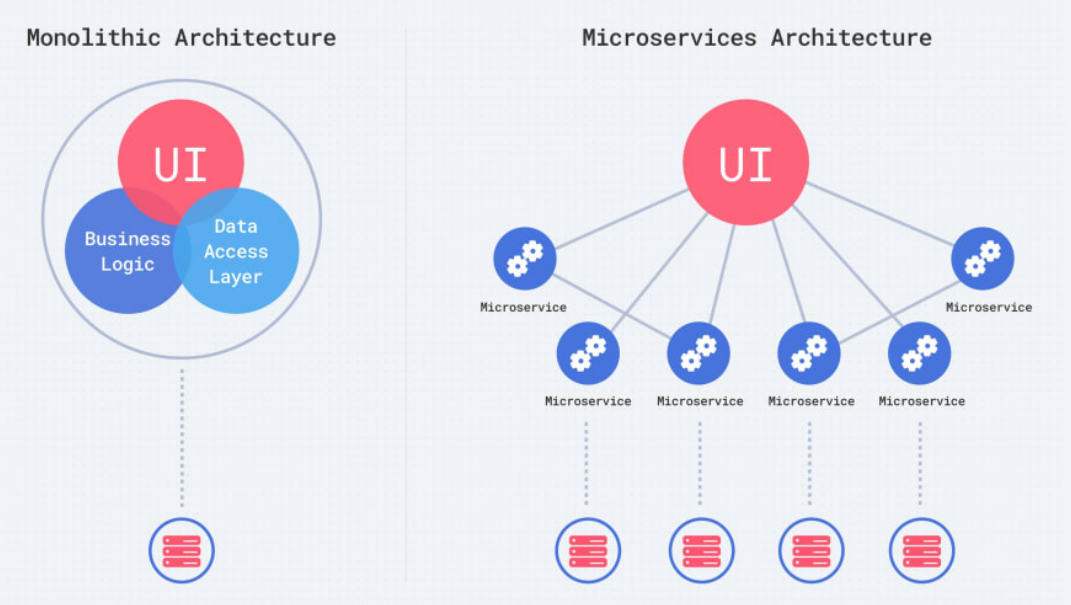
\includegraphics[width=0.5\textwidth]{monolithic-vs-microservices.png}
    \caption{Monolithic architecture vs Microservices architecture}
\end{figure}

\begin{figure}[H]
    \centering
    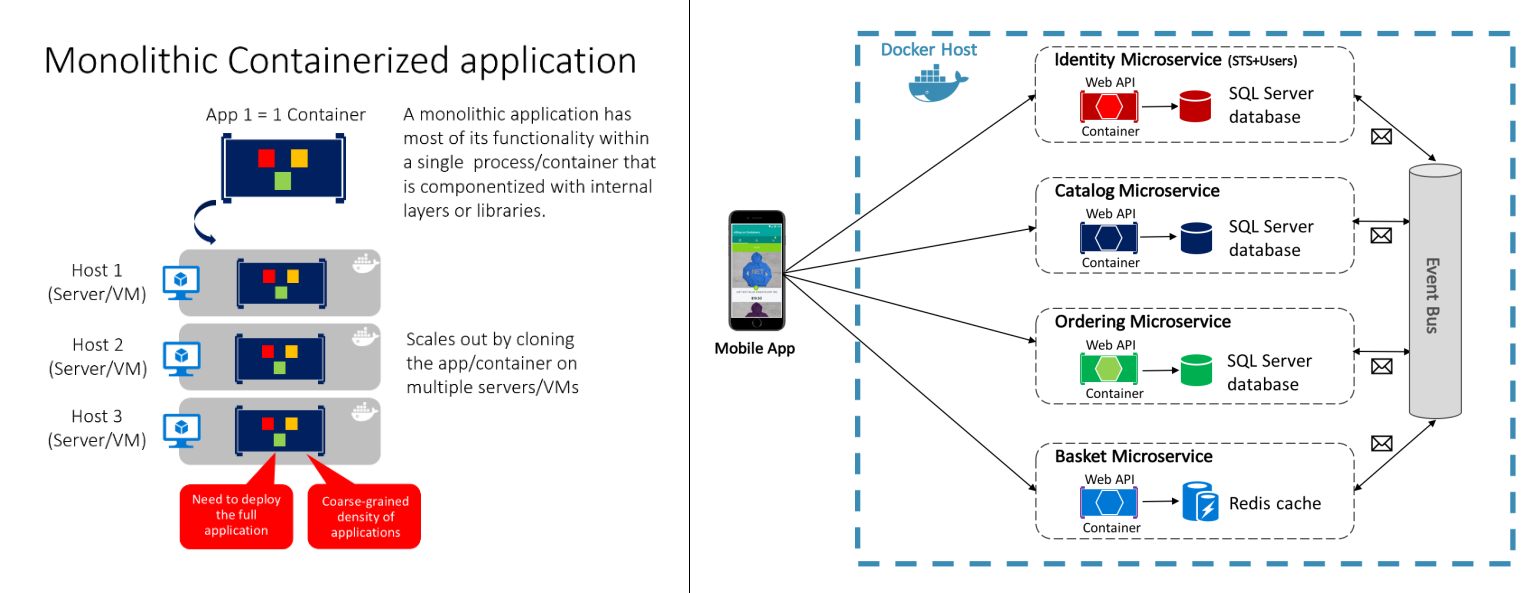
\includegraphics[width=0.5\textwidth]{monolithic-vs-microservices2.png}
    \caption{Monolithic Containerized application}
\end{figure}

Microservices does \bold{not} necessarily mean containerization!

\subsection{Virtualization vs Containerization}

\begin{figure}[H]
    \centering
    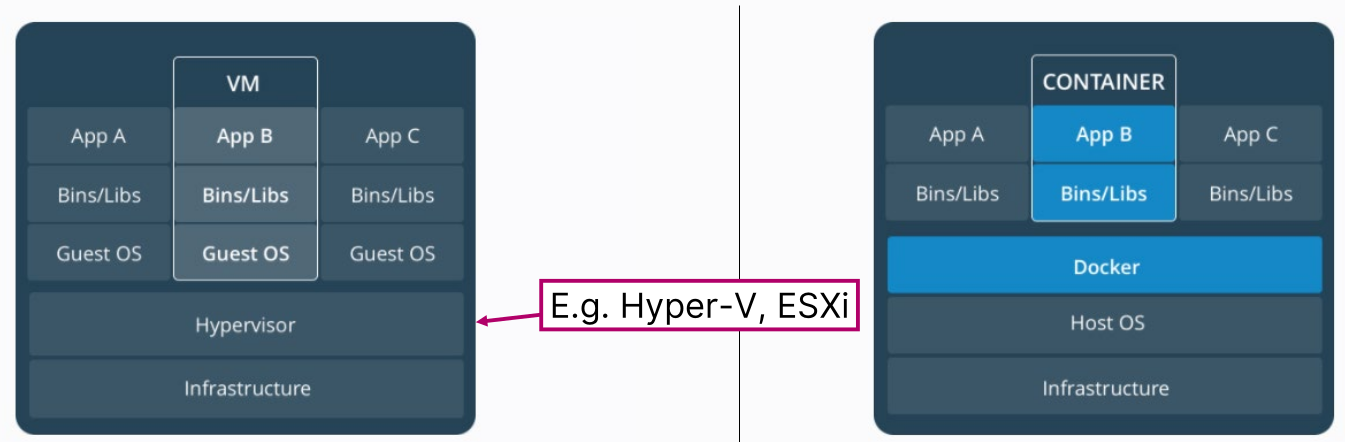
\includegraphics[width=0.5\textwidth]{virtualization-vs-containerization.png}
    \caption{Virtualization vs Containerization}
\end{figure}

\subsubsection{Virtualization}

\begin{itemize}
    \item = An abstraction of physical hardware turning one server into many servers
    \item Multiple VMs can run on the same machine
    \item Each VM includes a full copy of an Operating System (OS), one or more apps
    \item Takes a lot of space
    \item Can be slow to boot
\end{itemize}

\subsubsection{Containerization}

\begin{itemize}
    \item = An abstraction at the app layer that packages code and dependencies together
    \item Multiple containers can run on the same machine, they share the OS kernel with each other, each running as isolated processes in user space.
    \item Takes up less space than VMs
    \item Boot up almost instantly
\end{itemize}

\begin{figure}[H]
    \centering
    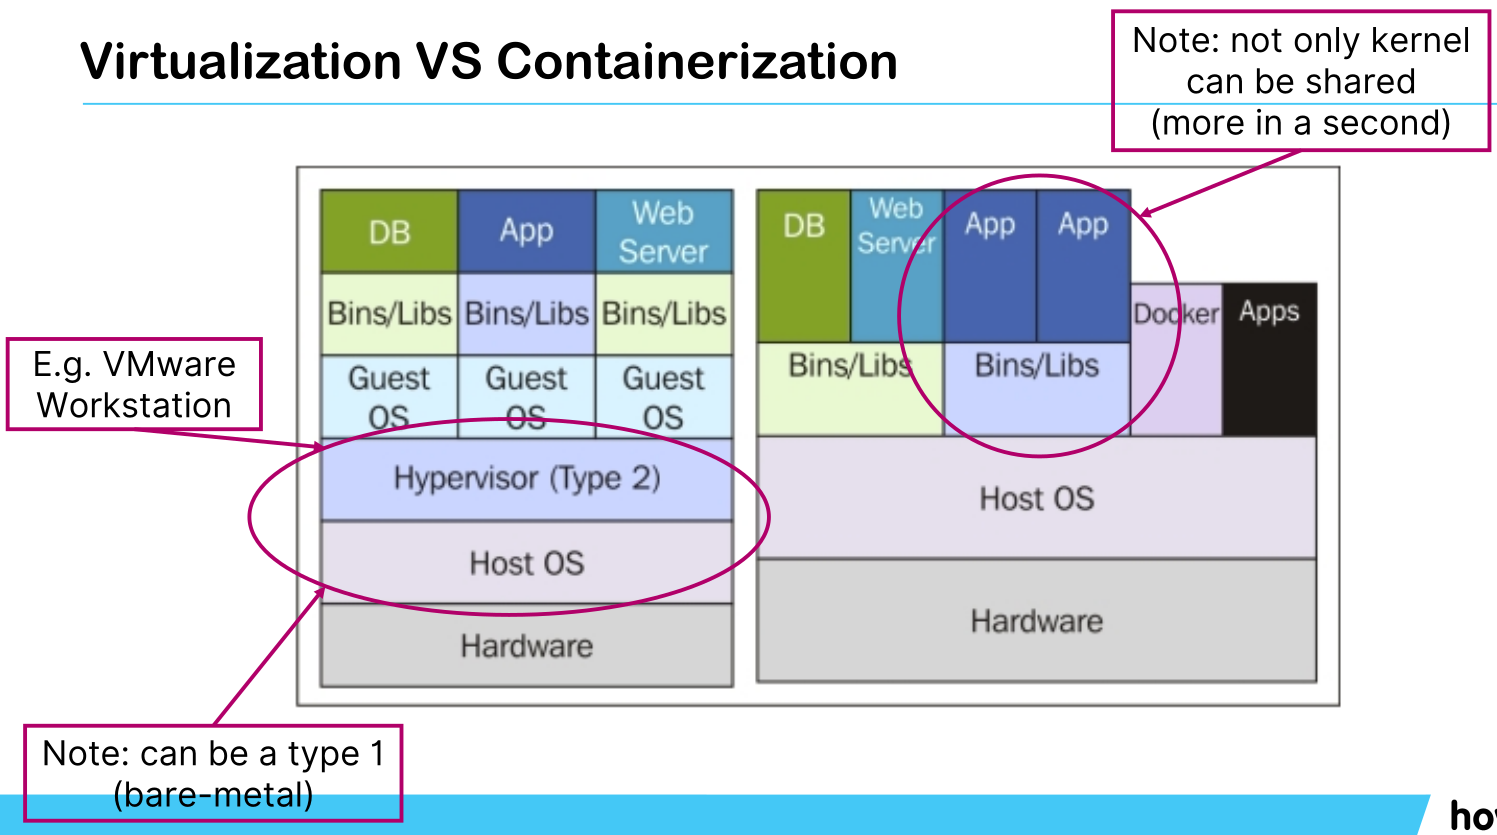
\includegraphics[width=0.5\textwidth]{virtualization-vs-containerization2.png}
    \caption{Schematic }
\end{figure}

\subsection{Shared kernel}

\subsubsection{What is a kernel?}

\begin{itemize}
    \item Piece of software that offers basic functionality to the OS
    \item System calls: open, read, write, close, wait, exit, \dots
    \item A typical kernel has a few hundred system calls
\end{itemize}

\begin{figure}[H]
    \centering
    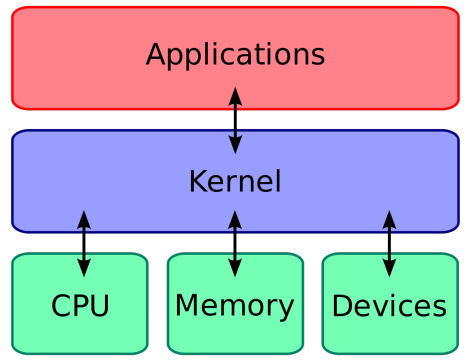
\includegraphics[width=0.3\textwidth]{kernel.png}
    \caption{The kernel is the layer that communicates between hardware and applications}
\end{figure}


\begin{itemize}
    \item Docker shares the host OS kernel
    \begin{itemize}
        \item Host OS: Windows / MacOS / Linux
        \item Shared Linux Kernel
    \end{itemize}
\end{itemize}

\begin{figure}[H]
    \centering
    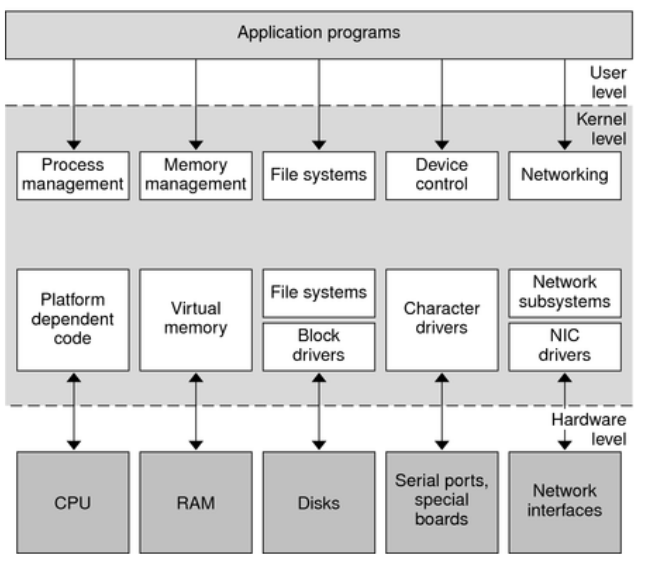
\includegraphics[width=0.5\textwidth]{kernel2.png}
    \caption{Kernel in detail}
\end{figure}

\begin{itemize}
    \item The Ubuntu container requires the Linux kernel
    \item The Linux kernel runs in a Virtual Machine
\end{itemize}

\begin{figure}[H]
    \centering
    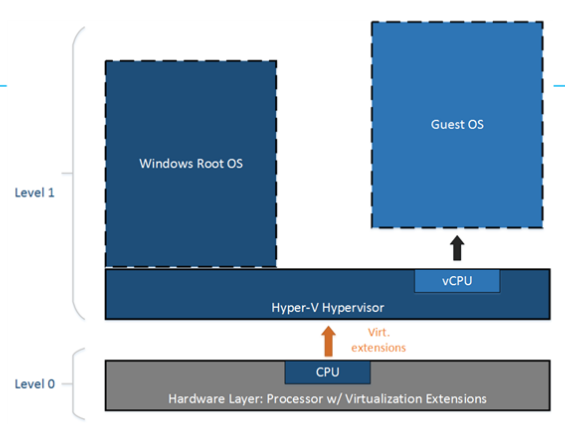
\includegraphics[width=0.45\textwidth]{kernel3.png}
    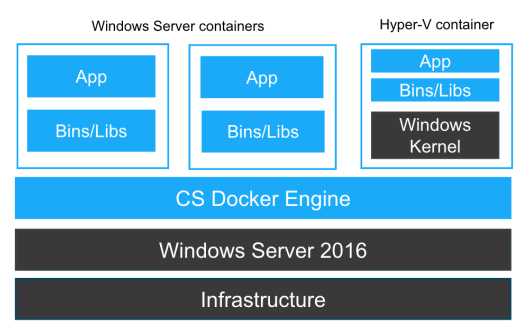
\includegraphics[width=0.45\textwidth]{kernel4.png}
    \caption{}
\end{figure}

\subsubsection{How?}

Two important Linux kernel features:

\begin{itemize}
    \item \bold{Namespaces} are a feature of the Linux kernel that partitions kernel resources
    \item \bold{cgroups} (control croups) is a Linux kernel feature that limits, accounts for, and isolates resource usage of a collection of processes 
\end{itemize}

Simpler:

\begin{itemize}
    \item Namespaces = isolating resources per process (or group of processes)
    \item cgroups = Limitating resource usage per process (or group of processes)
\end{itemize}

\subsubsection{Namespaces}

\begin{itemize}
    \item 7 types:
    \begin{itemize}
        \item mount, UTS, IPC, network, PID, cgroup, user
    \end{itemize} 
    \item For the process (or group of processes) it looks like there is a completely isolated set of resources
\end{itemize}

\subsubsection{Containers}

What is a container?

\begin{itemize}
    \item One or more running processes (if not running anymore $\Rightarrow$ container dead)
    \item Resources are specifically assigned to it
    \item The real bulding blocks: Linux kernel features
    \begin{itemize}
        \item Namespaces
        \item cgroups
    \end{itemize}
\end{itemize}

\subsection{Images}

What is an image?

\begin{itemize}
    \item Filesystem snapshot
    \item Startup command
    \item Layered structure \bold{\textcolor{red}{(!)}}
\end{itemize}

Instance of image = container

\subsubsection{Image layer}

\begin{figure}[H]
    \centering
    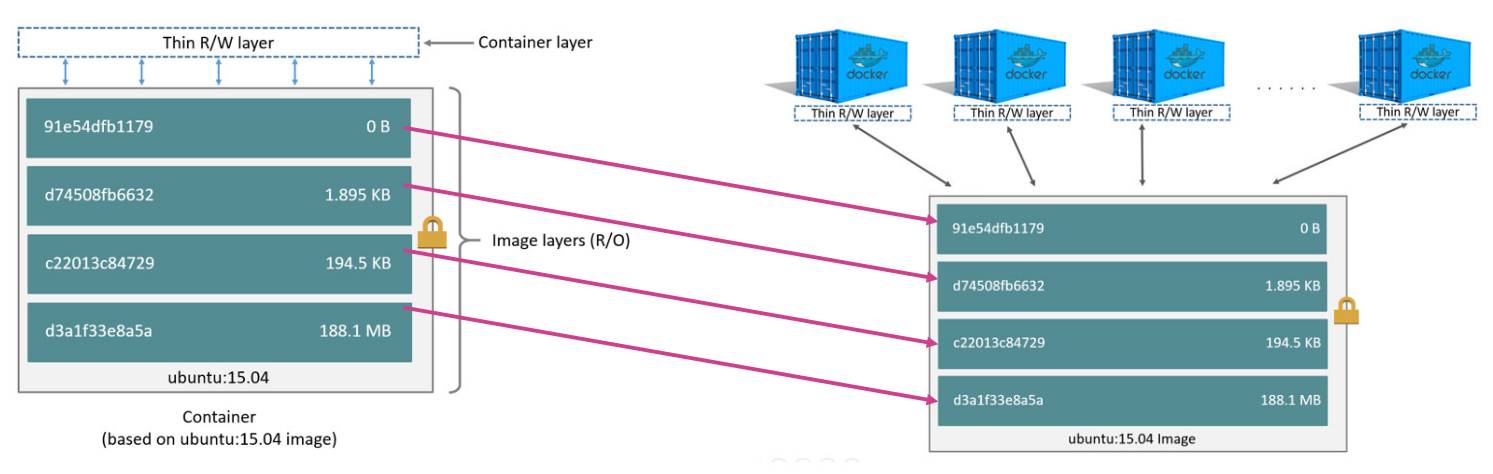
\includegraphics[width=0.8\textwidth]{image-layers.png}
    \caption{Image layers}
\end{figure}

\begin{itemize}
    \item RUN, COPY, ADD
    \begin{itemize}
        \item = new read-only layer
    \end{itemize}
    \item Top layer = container layer
    \begin{itemize}
        \item Writeable
    \end{itemize}
    \item Delete container = delete container layer
    \begin{itemize}
        \item Image will still exist
        \item Peristent volumes
    \end{itemize}
\end{itemize}


\subsection{Docker is lightweight}

\begin{itemize}
    \item Shared kernel
    \item Container has no OS
    \item Less disk space $\Rightarrow$ sharing layers
    \item Small community images
    \begin{itemize}
        \item ex: Alpine Linux (small, simple, secure)
    \end{itemize}
    \item Current Docker version is using runC (previously LXC = Linux Containers)
    \begin{itemize}
        \item runC = tooling (written in Go) that makes it possible to create and run containers
        \item runC = CLI to `easily' access kernel features such as cgroups and namespacing
        \item runC = successor of libcontainer (developed by Docker)
        \item Open-sourced $\Rightarrow$ better community
        \item runC implements `Open Container Initiative Runtime Specification'
        \item \url{https://github.com/opencontainers/runtime-spec}
    \end{itemize}
\end{itemize}

Docker is `nothing more' than an ecosystem about creating \& running containers

\subsection{Using Docker}

(see slides 40-55 in \underline{02\_big\_data\_01\_containers.pdf})



\end{document}